\documentclass[a4paper,UTF8]{article}
\usepackage{ctex}
\usepackage[margin=1.25in]{geometry}
\usepackage{color}
\usepackage{graphicx}
\usepackage{amssymb}
\usepackage{amsmath}
\usepackage{amsthm}
\usepackage{enumerate}
\usepackage{bm}
\usepackage{hyperref}
\usepackage{epsfig}
\usepackage{color}
\usepackage{mdframed}
\usepackage{lipsum}
\usepackage{tcolorbox}
\usepackage{graphicx}
\newmdtheoremenv{thm-box}{Theorem}
\newmdtheoremenv{prop-box}{Proposition}
\newmdtheoremenv{def-box}{定义}

\usepackage{listings}
\usepackage{xcolor}
\lstset{
	numbers=left, 
	numberstyle= \tiny, 
	keywordstyle= \color{ blue!70},
	commentstyle= \color{red!50!green!50!blue!50}, 
	frame=shadowbox, % 阴影效果
	rulesepcolor= \color{ red!20!green!20!blue!20} ,
	escapeinside=``, % 英文分号中可写入中文
	xleftmargin=2em,xrightmargin=2em, aboveskip=1em,
	framexleftmargin=2em
} 

\usepackage{booktabs}

\setlength{\evensidemargin}{.25in}
\setlength{\textwidth}{6in}
\setlength{\topmargin}{-0.5in}
\setlength{\topmargin}{-0.5in}
% \setlength{\textheight}{9.5in}
%%%%%%%%%%%%%%%%%%此处用于设置页眉页脚%%%%%%%%%%%%%%%%%%
\usepackage{fancyhdr}                                
\usepackage{lastpage}                                           
\usepackage{layout}                                             
\footskip = 12pt 
\pagestyle{fancy}                    % 设置页眉                 
\lhead{2020年春季}                    
\chead{机器学习导论}                                                
% \rhead{第\thepage/\pageref{LastPage}页} 
\rhead{作业二}                                                                                               
\cfoot{\thepage}                                                
\renewcommand{\headrulewidth}{1pt}  			%页眉线宽,设为0可以去页眉线
\setlength{\skip\footins}{0.5cm}    			%脚注与正文的距离           
\renewcommand{\footrulewidth}{0pt}  			%页脚线宽,设为0可以去页脚线

\makeatletter 									%设置双线页眉                                        
\def\headrule{{\if@fancyplain\let\headrulewidth\plainheadrulewidth\fi%
\hrule\@height 1.0pt \@width\headwidth\vskip1pt	%上面线为1pt粗  
\hrule\@height 0.5pt\@width\headwidth  			%下面0.5pt粗            
\vskip-2\headrulewidth\vskip-1pt}      			%两条线的距离1pt        
 \vspace{6mm}}     								%双线与下面正文之间的垂直间距              
\makeatother  

%%%%%%%%%%%%%%%%%%%%%%%%%%%%%%%%%%%%%%%%%%%%%%
\numberwithin{equation}{section}
%\usepackage[thmmarks, amsmath, thref]{ntheorem}
\newtheorem{theorem}{Theorem}
\newtheorem*{definition}{Definition}
\newtheorem*{solution}{Solution}
\newtheorem*{prove}{Proof}
\newcommand{\indep}{\rotatebox[origin=c]{90}{$\models$}}

\usepackage{multirow}

%--

%--
\begin{document}
\title{机器学习导论\\
作业二}
\author{学号, 作者姓名, 邮箱}
\maketitle

\section{[15 pts] Linear Regression}
给定数据集$D=\{(\mathbf{x}_i,y_i)\}_{i=1}^m$,最小二乘法试图学得一个线性函数$y=\mathbf{w^*}\mathbf{x}+b^*$使得残差的平方和最小化,即
\begin{equation}
	(\mathbf{w^*},b^*) = \mathop{\arg\min}_{\mathbf{w},b} \sum_{i=1}^m [y_i-(\mathbf{w}\mathbf{x_i}+b)]^2 . 
\end{equation}
“最小化残差的平方和”与“最小化数据集到线性模型的欧氏距离之和”或是“最小化数据集到线性模型的欧氏距离的平方和”一致吗?考虑下述例子
\begin{equation}
	D = \{ (-1,0) , (0,0) , (1,1) \} , 
\end{equation}
并回答下列问题。

\begin{enumerate}[(1)]
	\item \textbf{[5 pts]} 给出“最小化残差的平方和”在该例子中的解$(w^*,b^*)$。
	\item \textbf{[5 pts]} 给出“最小化数据集到线性模型的欧氏距离的平方和”在该例子中的数学表达式,并给出其解$(w_{E},b_{E})$,该解与$(w^*,b^*)$一致吗?
	\item \textbf{[5 pts]} 给出“最小化数据集到线性模型的欧氏距离之和”在该例子中
	的数学表达式,$(w^*,b^*)$是该问题的解吗?
\end{enumerate}

\begin{solution}
此处用于写解答(中英文均可)
\begin{enumerate}[(1)]
\item
\begin{equation*}
\begin{split}
	\text{设} E(w,b)=\sum_{i=1}^m [y_i-(\mathbf{w}\mathbf{x_i}+b)]^2\\
	\frac{\partial E(w,b)}{\partial w} = 2\left((w \sum_{i=1}^m x_i^2- \sum_{i=1}^m(y_i-b)x_i)\right)\\
	\frac{\partial E(w,b)}{\partial b} = 2\left(mb-\sum_{i=1}^m(y_i-wx_i)\right)\\
	\text{令以上两式为0可以解得}\\
	w^* = \frac{\sum_{i=1}^m y_i(x_i-\bar{x})}{\sum_{i=1}^mx_i^2-\frac{1}{m}\left(\sum_{i=1}^m x_i\right)^2}=\frac{1}{2}\\
	b^* = \frac{1}{m} \sum_{i=1}^m(y_i-wx_i)=\frac{1}{3}\\
	\text{其中 } \bar{x}=\frac{1}{m} \sum_{i=1}^m x_i
\end{split}
\end{equation*}
\item
\begin{equation*}
\begin{split}
	(w_E,b_E) &= argmin \sum_{i=1}^m \frac{(wx_i+b-y_i)^2}{1+w^2}\\
	&=argmin\left( \frac{3b^2-2b+2w^2-2w+1}{1+w^2}	\right)\\
	& b_E = \frac{1}{3}\ w_E = \frac{\sqrt{13}-2}{3} \text{ 并不一致}
\end{split}
\end{equation*}
\item 
\begin{equation*}
	\begin{split}
		(w^*,b^*) &= argmin \sum_{i=1}^m \frac{| wx_i+b-y_i |}{\sqrt{1+w^2}}\\
		& = argmin \left(\frac{|b-w|+|b|+|b+w-1|}{\sqrt{w^2+1}}\right) \\
		& if\ b\ge w\ and\ b\ge 1-w, b^* = \frac{1}{2},\ m^*=\frac{1}{2},\ ans=\frac{\sqrt{5}}{5}\\
		& if\ b\ge w\ and\ b\le 1-w, b^*=0,\ m^*=0,\ ans=1\\
		& if\ b\le w\ and\ b\ge 1-w, b^*=0,\ m^*=1,\ ans=\frac{\sqrt{2}}{2}\\
		& if\ b\le w\ and\ b\le 1-w, b^*=\frac{1}{2},\ m^*=\frac{1}{2},ans=ans=\frac{\sqrt{5}}{5}\\
		&\therefore b*=\frac{1}{2},m^*=\frac{1}{2},\text{ 并不相同,bu}
	\end{split}
\end{equation*}
\end{enumerate}
\end{solution}

\section{[40+5 pts] 编程题, Logistic Regression}
\textbf{请结合编程题指南进行理解}
\par 试考虑对率回归与线性回归的关系。最简单的对率回归的所要学习的任务仅是根据训练数据学得一个$\beta=(\omega;b)$,而学习$\beta$的方式将有下述两种不同的实现:
\par 0. [闭式解] 直接将分类标记作为回归目标做线性回归,其闭式解为 \begin{equation}
	\beta=({\hat{X}}^T\hat{X})^{-1}\hat{X}^Ty
	\end{equation}, 其中$\hat{X}=(X;\vec{1})$

\par 1. [数值方法] 利用牛顿法或梯度下降法解数值问题
\begin{equation}
	\min_{\mathbf{\beta}} \sum_{i=1}^{m}(-y_i\beta^T\hat{x_i}+\ln (1+e^{\beta^T\hat{x_i}})). 
\end{equation}
得到$\beta$后两个算法的决策过程是一致的,即:
\begin{enumerate}[(1)]
	\item $z=\beta X_{i}$
	\item $f=\frac{1}{1+e^{-z}}$
	\item 决策函数\begin{equation}
		y_{i}=
		\begin{cases}
		1,&\mbox{if $f>\theta$}\\
		0,&\mbox{else}
		\end{cases}
		\end{equation}
	\end{enumerate}
	其中$\theta$为分类阈值。回答下列问题:
	\begin{enumerate}[(1)]
		\item \textbf{[10 pts]} 试实现用闭式解方法训练分类器。若设分类阈值$\theta=0.5$,此分类器在Validation sets下的准确率、查准率、查全率是多少?
		\item \textbf{[10 pts]} 利用所学知识选择合适的分类阈值,并输出闭式解方法训练所得分类器在test sets下的预测结果。
		\item \textbf{[10 pts]} 利用数值方法重新训练一个新的分类器。若设分类阈值$\theta=0.5$,此分类器在Validation sets下的准确率、查准率、查全率是多少?
		\item \textbf{[10 pts]} 利用所学知识选择合适的分类阈值,并输出数值方法训练所得分类器在test sets下的预测结果。
		\item \textbf{[选做][Extra 5 pts]} 谈谈两种方法下分类阈值的变化对预测结果的影响,简要说明看法。
	\end{enumerate}
\begin{solution} 此处用于写解答(中英文均可)
	\begin{enumerate}[(1)]
		\item 准确率:0.74,查准率:0.67,查全率:1.0
		\item 在[0,1]区间上进行步长为0.002的线性搜索,得到最优$\theta$值为0.516,依据为acc+p+r。完整的度量与$\theta$取值关系如图
			  \\ 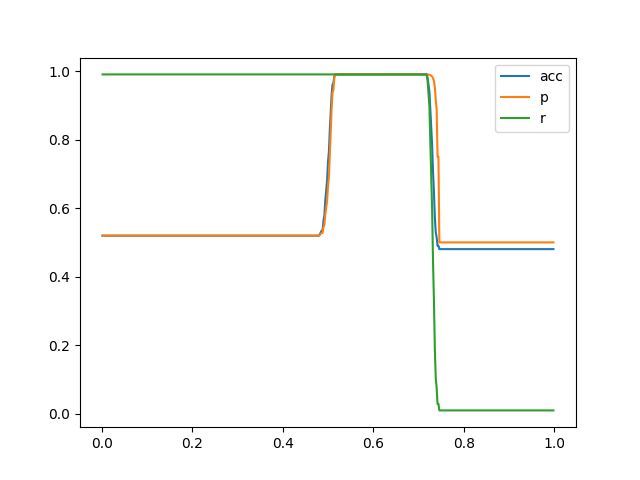
\includegraphics[scale=0.8]{figure/0_graph.png}
		\item 本问使用牛顿法。准确率:1.0,查准率:1.0,查全率:1.0
		\item 因为三个率都较高,且在相当大区间内都无变化,于是改为在[0,1]区间对数尺度上进行线性搜索,横坐标为1e-x,得到最优$\theta$为0.05,判断依据是acc+p+r\\
			  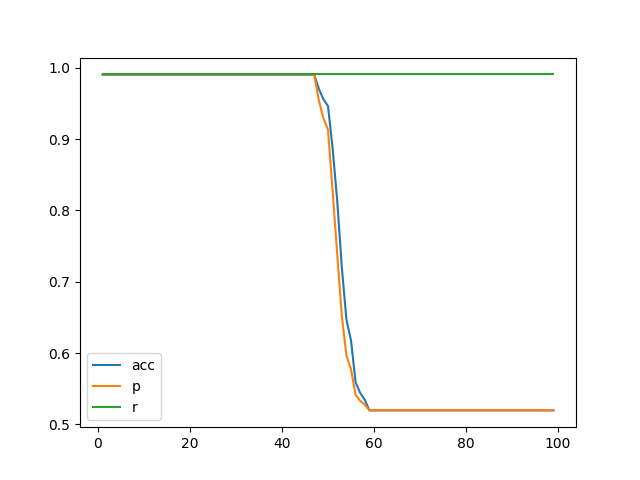
\includegraphics[scale=0.8]{figure/1_graph.png}
		\item 通过在程序中直接增加输出我们可以发现,闭式解方法的$\beta$的模远远小于牛顿法优化得到的$\beta$。由于sigmoid函数中含有$e^{-z}$项在分母上,而$z=\beta X$关于不同X的变化幅度与$\beta$模长正相关
			  因此拥有较小模长的闭式解方法输出的f分布将相对紧凑,而数值优化得到的f分布将更分散,因此改变$\theta$的大小,闭式解方法将相对更加敏感,产生的影响更大。
	\end{enumerate}
\end{solution}

\section{[10 pts] Linear Discriminant Analysis}
在凸优化中,试考虑两个优化问题,如果第一个优化问题的解可以直接构造出第二个优化问题的解,第二个优化问题的解也可以直接构造出第一个优化问题的解,则我们称两个优化问题是等价的。基于此定义,试证明优化问题\textbf{P1}与优化问题\textbf{P2}是等价的。
\begin{equation}
	\label{P1}
	\max_{\mathbf{w}} \frac{\mathbf{w}^\top S_b \mathbf{w}}{\mathbf{w}^\top S_w \mathbf{w}} . 
\end{equation}
\begin{equation}
	\label{P2}
	\begin{aligned}
		\min_{\mathbf{w}} & \quad -\mathbf{w}^\top S_b \mathbf{w} \\ 
		\text{s.t.} & \quad \mathbf{w}^\top S_w \mathbf{w} = 1 . 
	\end{aligned}
\end{equation}

\begin{solution} 此处用于写解答(中英文均可)\\
	若$w_1$是问题(3.1)的解,则$\frac{w_1^T}{\sqrt{w_1^T S_w w}} S_w \frac{w_1}{\sqrt{w_1^T S_w w}}=1$, 且由$w_1=\max_{\mathbf{w}} \frac{\mathbf{w}^\top S_b \mathbf{w}}{\mathbf{w}^\top S_w \mathbf{w}}$
	可知$\frac{w_1^T}{\sqrt{w_1^T S_w w}} S_b \frac{w_1}{\sqrt{w_1^T S_w w}} = max_w(w^TS_bw)=min_w(-w^TS_bw)$. 所以$\frac{w_1}{\sqrt{w_1^T S_w w}}$是问题(3.2)的解\\
	若$w_2$是问题(3.2)的解,同理易见其也是问题(3.1)的解,且任意问题(3.1)的解$w,aw$也是问题(3.1)的解
	\\ 综上,问题(3.1)与(3.2)等价
\end{solution}
\section{[35 pts] Multiclass Learning}
在处理多分类学习问题的时候,我们通常有两种处理思路:一是间接求解,利用一些基本策略(OvO, OvR, MvM)将多分类问题转换为二分类问题,进而利用二分类学习器进行求解。二是直接求解,将二分类学习器推广到多分类学习器。
\subsection{问题转换}
\begin{enumerate}[(1)]
	\item \textbf{[5 pts]} 考虑如下多分类学习问题:假设样本数量为$n$,类别数量为$C$,二分类器对于大小为$m$的数据训练的时间复杂度为$ \mathcal{O}(m) $(比如利用最小二乘求解的线性模型)时,试分别计算在OvO、OvR策略下训练的总时间复杂度。
	\item \textbf{[10 pts]} 当我们使用MvM处理多分类问题时,正、反类的构造必须有特殊的设计,一种最常用的技术为“纠错输出码”(ECOC),根据阅读材料(\href{ccs.neu.edu/home/vip/teach/MLcourse/4_boosting/lecture_notes/ecoc/ecoc.pdf}{Error-Correcting Output Codes}、\href{https://arxiv.org/pdf/cs/9501101.pdf}{Solving Multiclass Learning Problems via Error-Correcting Output Codes}\cite{dietterich1994solving};前者为简明版,后者为完整版)回答下列问题:
	\begin{enumerate}[1)]
		\item 假设纠错码之间的最小海明距离为$n$,请问该纠错码至少可以纠正几个分类器的错误?对于图\ref{img}所示的编码,请计算该纠错码的最小海明距离并分析当两个分类器出错时该编码的纠错情况。
		\begin{figure}[htbp]
			\centering
			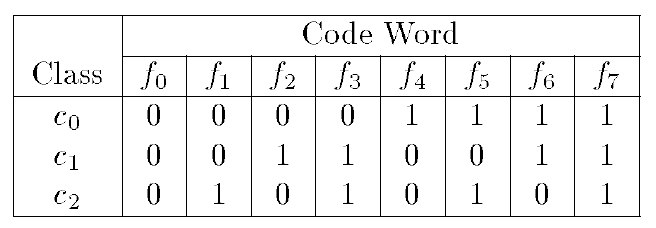
\includegraphics[width=.8\textwidth]{figure/codeword.png} %1.png是图片文件的相对路径
			\caption{3类8位编码} %caption是图片的标题
			\label{img} %此处的label相当于一个图片的专属标志,目的是方便上下文的引用
		\end{figure}
		\item 令码长为8,类别数为4,试给出海明距离意义下的最优ECOC编码,并简述构造思路。
		\item 试简述好的纠错码应该满足什么条件?(请参考完整版阅读资料)
		\item ECOC编码能起到理想纠错作用的重要条件是:在每一位编码上出错的概率相当且独立,试分析多分类任务经ECOC编码后产生的二类分类器满足该条件的可能性及由此产生的影响。
	\end{enumerate}	
	\item \textbf{[10 pts]} 使用OvR和MvM将多分类任务分解为二分类任务求解时,试论述为何无需专门这对类别不平衡进行处理。
\end{enumerate}
\subsection{模型推广}
\textbf{[10 pts]} 对数几率回归是一种简单的求解二分类问题的广义线性模型,试将其推广到多分类问题上,其中标记为$y\in\{1,2\dots,K\}$。

提示:考虑如下$K-1$个对数几率
$$\ln\frac{p(y=1|\mathbf{x})}{p(y=K|\mathbf{x})},	\ln\frac{p(y=2|\mathbf{x})}{p(y=K|\mathbf{x})},\cdots,	\ln\frac{p(y=K-1|\mathbf{x})}{p(y=K|\mathbf{x})}$$

\begin{solution} 此处用于写解答(中英文均可)\\
	4.1
	\begin{enumerate}[(1)]
		\item	OvO: $T_{OvO} = \frac{C(C-1)}{2} O(2\frac{n}{C}) = O((C-1)n)=O(Cn)$\\
				OvR: $T_{OvR} = C O(n) = O(Cn)$
		\item  
		\begin{enumerate}[1)]
			\item 最小海明距离为n,则至少可纠正$\lfloor \frac{n-1}{2} \rfloor$个分类器的错,因为改变输出编码的任意$\lfloor \frac{n-1}{2} \rfloor$位,将不能足以使测试样本的海明距离离某个错误分类比原本的正确分类近。\\
				  图中$d_{01}=4,d_{12}=4,d_{20}=4$,故最小海明距离为4,当两个分类器出错时,$\lfloor \frac{4-1}{2} \rfloor = 1 < 2$, 因此不能纠错,但是可以检测到出错。
			\item 参考简略版论文,在类别较小的时候可以采用Exhaustive code的方式进行设计,不过这里要求的码长为8,比标准Exhaustive code要多一位。
				  构造思路是依次使用2的降序幂次个1与0的间隔序列构造每一个类的编码,构造的结果为:\\ c0:11111111 c1:00001111 c2:00110011 c3:01010101\\
				  这样构造的ECOC编码同时兼具下面会具体讲到的row seperation 与 column separation,是最佳的ECOC码
			\item 1.Row Seperation:任何一个编码序列使用汉明距离应该良好可分到某个类
				  \\2.Column Seperation:每个位置的编码(每个分类器)与其余位置编码不相关,即与其他位置的编码以及其取反结果的汉明距离应尽可能大
			\item 由于保证了Column Seperation,ECOC编码的每一位尽可能不相关,即每一个分类器尽可能不相关,因此他们在分类出错情况上也应该有较低的相关性,因此能较好的满足每一位上编码出错的概率独立的假设。至于每一位上出错概率,因为使用相同算法所以算法导致的分类误差相当,由于对数据集中的每一个类其被划分的情况是公平的,由划分导致的误差将相互抵消,因此每一位编码上出错率相当的假设也成立。综上,使用ECOC编码后将能较好的提供针对各类的大致相当的正确分类能力和一定纠错能力。
			\end{enumerate}
			\item 虽然OvO与MvM中确实存在很显然的类别不平衡,不过划分的方法已经确定了这种不平衡对么一个(组)类别都会均等出现,因此类别不平衡产生的影响是相互抵消的,总体上基本是平衡的,因此一般无需专门处理。
	\end{enumerate}
	4.2 分别训练k-1个二分类器(或认为w与b从标量变成了向量),使得$\ln\frac{p(y=i|\mathbf{x})}{p(y=K|\mathbf{x})}=w_i^Tx+b_i,i=1,2 \dots k-1.$ 则$p(y=i|x)=e^{w_i^Tx+b_i}p(y=K|x)$, 将概率归一化处理产生$p(y=K|x)$后可得$p(y=i|x)=\frac{e^{w_i^Tx+b_i}}{\sum\limits_{j \in K}e^{w_j^Tx+b_j}},i=1,2\dots K.$ 此时进行判断的依据即针对输入数据分别求其属于每个类别的概率,并将概率最大的类别作为预测分类输出。
		至于训练方法,可以采取牛顿法或梯度下降法对w与b的每一维仍旧采用与二分类类似的优化方法优化得到。
\end{solution}
\bibliographystyle{plain}
\bibliography{ref.bib}
\end{document}